\graphicspath{{chapters/IGVimages/}}

\chapter*{IGV (Integrative Genomics Viewer)}

\section*{Main characteristics}
The human genome nowadays is being explored extensively thanks to the collection
of exome and whole-genome sequencing, epigenetic surveys, expression profiling
of coding and noncoding RNAs, single nucleotide polymorphism (SNP) and copy
number profiling, and functional assays. Those findings are essential to pave the way for the future precision medicine. This is an approach
for desease treatment and prevention that takes into account individual
variability in genes, environemtn, and lifestyle for each person. The right
drug, at the right time and at the right dose for each individual. 

\begin{figure}
    \caption{All the important elements to navigate into IGV are reported in the figure}
    \centering
    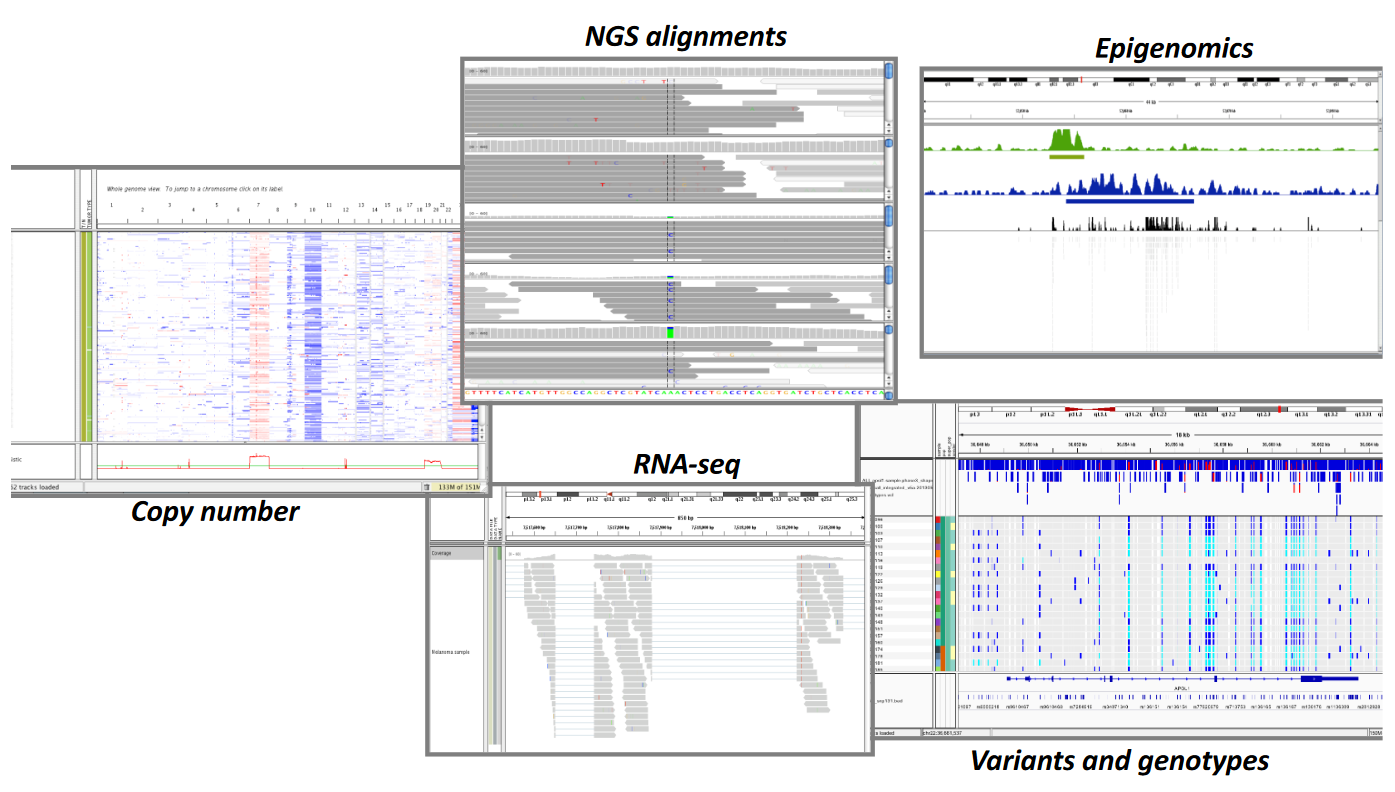
\includegraphics[width=0.6\textwidth]{usagesIGV.PNG}
    \label{IGVsee}
\end{figure}

The IGV software is an high-performance lightweight visualization tool for interactive exploration
of large, integrated genomic datasets. It supports a wide variety of data types,
including next-generation sequence data, and genomic annotations.

It allows to move, zoom in and out quickly over all genomic scales, and also to
jump in precise positions of the sequence. BAM files, which are read by IGV,
enable the retrieval of data for precise positions inside a chromosome. Pixel
resolution errors, occuring when if data density exceeds the constraint given by
the number of pixels available for display, could be solved through data
aggregation. As the user zooms below the ~50 kb range, individual aligned reads
become visible. It is possible then to zoom further, and see the bases at each
position

Data sets can be loaded from local or remote sources, including cloud-based
resources. 

Other information are present at
\href{https://authors.library.caltech.edu/72234/2/nbt.1754-S1.pdf}{Supplementaty
information - Integrative Genomics Viewer} pdf file

\begin{figure}
    \caption{All the important elements to navigate into IGV are reported in the figure}
    \centering
    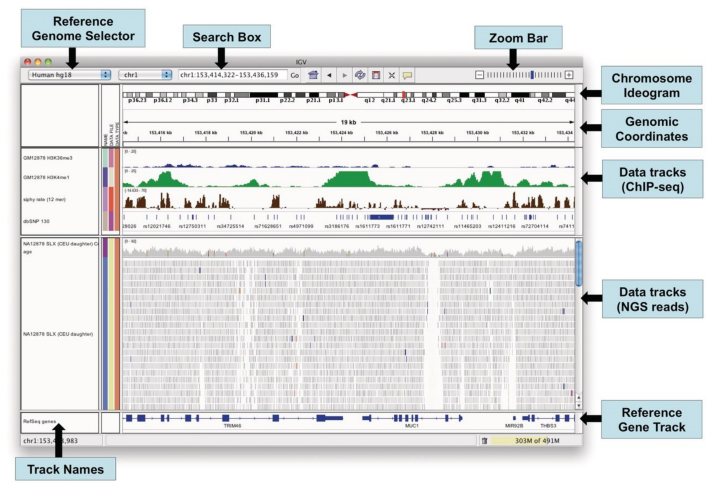
\includegraphics[width=0.6\textwidth]{IGVview.PNG}
    \label{IGVsee}
\end{figure}
\begin{figure}
    \caption{}
    \centering
    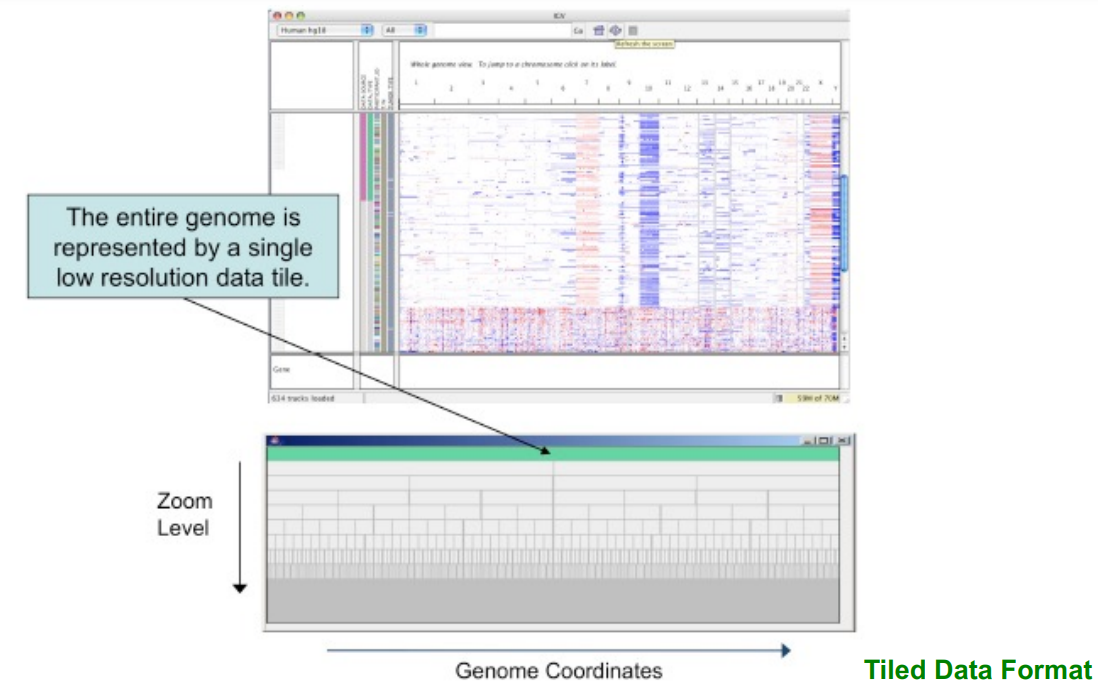
\includegraphics[width=0.6\textwidth]{Tiles.PNG}
    \label{Til}
\end{figure}l 

\begin{figure}
    \caption{}
    \centering
    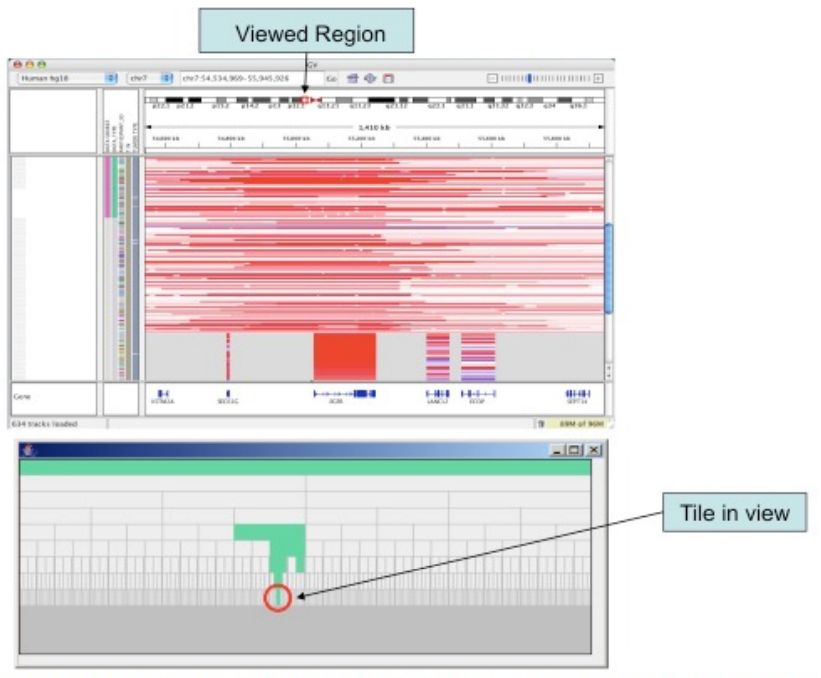
\includegraphics[width=0.6\textwidth]{TileView.PNG}
    \label{img: TileV}
\end{figure}

For each resolution scale (“zoom level”), the aggregated data is divided into
tiles that correspond to a region viewable on a typical user display \ref{TileV}. 

% \begin{figure}[h]
% \caption{in correspondance to SNP lower coverage}
% \centering
% \includegraphics[width=0.6\textwidth]{example}
% \label{}
% \end{figure}

%#TODO For each resolution scale (“zoom level”), the aggregated data is divided into
%tiles that correspond to a region viewable on a typical user display. Each tile
%is subdivided into bins, with the width of a bin chosen to correspond to the
%width represented by a pixel at that resolution scale. During the
%pre-computation step, data in each bin is aggregated into one or more summary
%statistics as specified by the user. Data Format: the corresponding data tiles
%for each zoom level are stored in the binary Tiled Data Format, or TDF, which
%has been optimized for fast tile retrieval. - tile sizes for each zoom level
%are constant and small, - only the data needed to render the view at the
%resolution supported by the screen display. - a single tile at the lowest
%resolution (spanning the entire genome) has the same memory footprint as a tile
%at the very high zoom levels (might span only a few kilobases). Tiles no longer
%in view are discarded as needed to free memory. Navigation through a data set
%is similar to that of Google Maps, allowing the user to zoom and pan seamlessly
%across the genome at any level of detail from whole genome to base pair.

\begin{figure}
    \caption{}
    \centering
    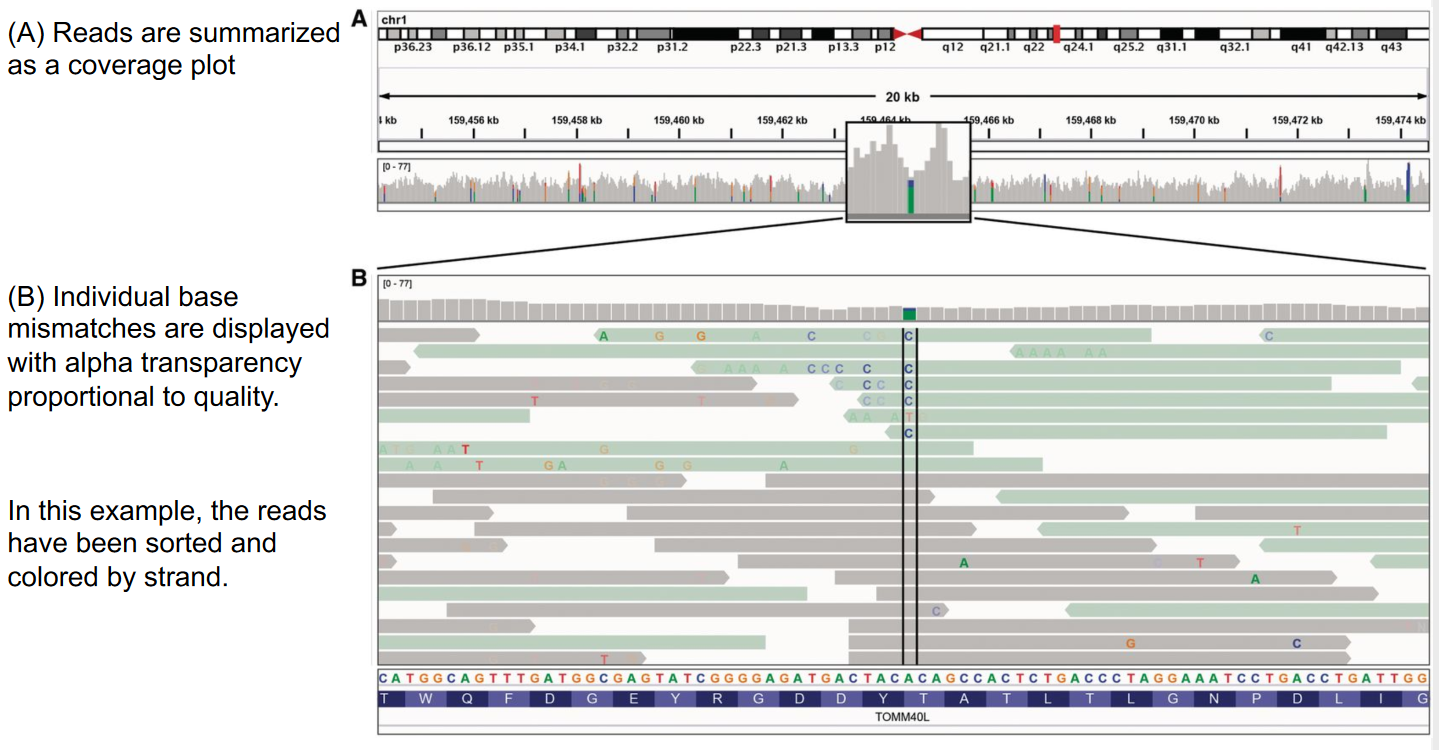
\includegraphics[width=0.6\textwidth]{IGVReadsView.PNG}
    \label{ViewReads}
\end{figure} 

\subsection*{Session Files}
Sessions are an integral part of IGV, allowing users to share their data and
views with other users simply and accurately. Session files describe the session
in XML.

\begin{figure}
    \caption{}
    \centering
    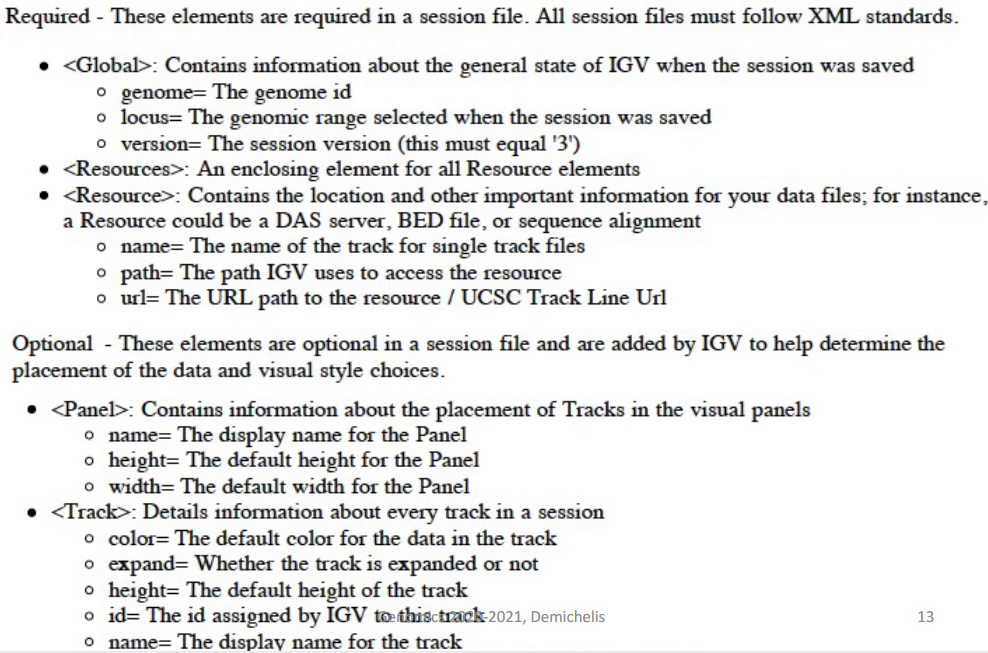
\includegraphics[width=0.6\textwidth]{structureXMLfile.PNG}
    \label{XMLfile}
\end{figure} 

\subsection*{Exercise}


EXERCISE
Reference genome in fasta file, annotations, and indexed
It is possible to see the single bases

- SNP1
heterozygous SNP

- SNP2
lower coverage
all the cytosines are on the reverse strand, could be associated to tachnical issues

% ----------------------

Paired-end reading, it is possible to understand if something strange happened to the sequence in the middle.
INVERSION
Drop in coverage on the sites of inversion
... (other cases already seen)

FIRST CASE chr1:11,043,245-11,061,901
Green reads
...

Healthy cells likely don't have tandem duplication. With perfect presence of a tumor sample. In this case, 1 of the alleles didn't undergo duplication, so why it's less than the 50\% 
Ploidy of cancer cells is an important characteristic
Purity of the sample is the portion of the sample that is tumor. Need to correct for this percentages.

SECOND CASE chr5:9,410,315-9,413,699
No coverage
Deletion on both the alleles, complete deletion of the portion

THIRD CASE chr7:31,576,117-31,599,940
No coverage in one part of the region
Inversion and an Hemyzigous deletion, it's not easy to understand what happened before and what after.
- 1st hypothesis: Inversiono first, Hemideletion second
Basically you have an inversion between B and F, and after the deletion of the ED portion, the other allele remains normal.

